\documentclass[11pt]{homework}
\usepackage[utf8]{inputenc}
\usepackage{graphicx}
\usepackage{wrapfig}
\usepackage[table]{xcolor}
\usepackage{biblatex}
\usepackage{abstract}
\addbibresource{bibliography.bib}
\renewcommand{\linespread}{1.0}

\begin{document}

\title{COMP-551 Mini-Project 2 \and COMP-551 Winter 2021}
\author{Arneet Singh Kalra, Behnaz Ghefati Feizabadi, Hussein Lakkis}
\date{February 28, 2021}
\maketitle{}

\begin{abstract}
\normalsize
The importance of machine learning algorithms in the field of Natural Language Processing and Text Classification is becoming more prominent now than ever. In this project, we investigated the performance of two  classification models on two benchmark datasets: the 20 News Group dataset as well as the IMDB Reviews set. More precisely, we implemented Naive Bayes (a generative model) from scratch and used Logistic Regression (a discriminative model) from the scikit-learn package. Furthermore, we implemented our own custom cross-validation to conduct hyper-parameter tuning to choose best values for our models. The datasets were also additionally tested using Scikit Learn's SGDC, Decision Tree, and Ada Boost classifiers. From our analysis, we conclude that for the 20 News Group dataset, the logistic regression approach achieved worse accuracy than Naive Bayes and was also significantly slower to train when compared to Naive Bayes. However, on the IMDB dataset, logistic regression was more accurate and faster to train. 
\end{abstract}

\section{Introduction}
\subsection{Project Background and Goals}
The goal of this project is to implement and compare  two text classification algorithms (Naive Bayes and Logistic Regression), using two well-known datasets, the Twenty News Group and IMDB Reviews. In addition to these models, we also chose to test them using Scikit Learn's SGDC (SVM), Binary Decision Tree, and Ada Boost classifiers. The 20 News Group Dataset is provided by Sklearn and contains textual data from newsgroup documents across twenty different newsgroups. The dataset itself was originally collected by Ken Lang for his paper, "Newsweeder: Learning to filter netnews", however it was never referenced in it \cite{Lang95}. The IMDB dataset contains data for movie reviews with ratings. The dataset was originally collected by a group of researchers at Stanford University to be used in their paper "Learning Word Vectors for Sentiment Analysis" published in 2011 \cite{maas-EtAl:2011:ACL-HLT2011}. We chose these datasets because they are well known benchmarking datasets. After the modeling, and based on the results of our analyses for both datasets, we conclude that Multinomial Naive Bayes is more accurate for the 20 News Group dataset. It is also almost 10 times faster to train than logistic regression. On the other hand, the IMDB dataset received the most accurate result from Logistic Regression, and was also faster using that model than Naive Bayes.

\subsection{Discussion of Related Work}
Our research on these datasets and modeling techniques led us to see various other applications as well as other algorithms for this task. A paper by Verma and Yenter describes their use of Convolutional Neural Networks and Long Short-term Memory Layers to do textual sentiment classification on the IMDB dataset. Their novel model boasts accuracies above 89\%, higher than our more accurate result, and can be applied on other datasets for sentimental analysis or text classification \cite{yenter2017deep}. Other sources showcase the wide range of real-life applications of using such modelling techniques. For example, Naive Bayes is commonly used as a filter to detect spam emails. A paper by Greek researches describes their work in using the dataset and developing various versions of the Naive Bayes models to increase the overall accuracy of detecting spam \cite{metsis2006spam}. Another paper from India presents the use of such techniques to determine the overall sentiment of a tweet posted by a Twitter user. Their research uses these models to predict the general sentiment based off words often used in tweets \cite{vadivukarassi2017sentimental}.

\section{Datasets}

\subsection{TFIDF Vectorizer}\label{TFDIF Vectorizer}
For both datasets, we used Scikit-Learn TFIDF Vectorizer to convert the textual data found in the sets to numerical features. This vectorizer specifically places less importance to words that appear often among all documents. We used the built-in "stop words" parameter of the vectorizer and set it to 'English' so that it ignores common words that are often not useful such as "and", "the", and "or". It also allows us to drop features that are noisy and lead to overfitting.

\subsection{20 News Group}
The 20 News Group dataset is a collection of approximately 20,000 newsgroup documents, partitioned fairly evenly across 20 different newsgroups, some of which are closely related while others have low correlation. We performed multi-class classification on the set to predict which of the 20 news groups is associated with a respective news document. While pre-processing the data, we first removed the header, footer, and quote features from the set to limit overfitting. Then we removed all punctuation, capital letters and numbers, and empty lines from the text documents.We also lower cased all words. After this, we used the TFIDF Vectorizer to convert the text features to numerical data. For this dataset, we set the vectorizer to exclude words that appear in less than 3 documents as it increases our accuracy. Our analysis showed that setting it to 3 resulted in a better result than the default of 1 document. Figures \ref{news-group-training-class-distribution} and \ref{news-group-testing-class-distribution} represent the class distribution analysis of our features for the training and testing sets respectively. There is no significant imbalance between the different classes for both sets, which is beneficial to the accuracy of our model.

\begin{figure}[h!]
  \centering
  \begin{minipage}[h]{0.3\textwidth}
    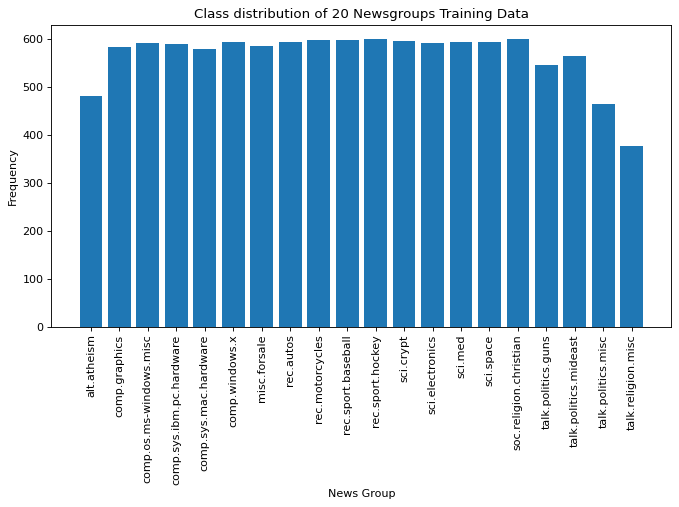
\includegraphics[width=\textwidth]{news-class-distribution-training.png}
    \caption{News Training Set Class Distribution}\label{news-group-training-class-distribution}
  \end{minipage}
\hspace{1.5cm}
    \begin{minipage}[h]{0.3\textwidth}
    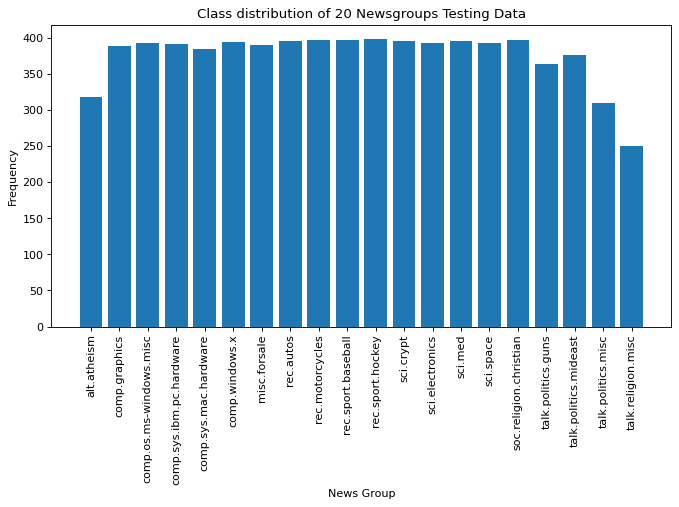
\includegraphics[width=\textwidth]{news-class-distribution-testing.png}
    \caption{News Testing Set Class Distribution}\label{news-group-testing-class-distribution}
  \end{minipage}
\end{figure}

\subsection{IMDB Reviews}
The IMDB Reviews dataset contains 50 000 reviews split evenly into training and testing sets. Alongside the reviews, a rating on 10 is given for the movie. This rating is translated to a positive class if it is between 7-10, or a negative class if it is below 5. A rating of 5 or 6 is ignored for the purposes of the analysis. We performed binary classification on the dataset to predict if a given review results in a positive or negative rating. During the preprocessing of the data, we removed text within '<>' brackets as well as any emoticons. We then used the TFIDF Vectorizer as outlined in \ref{TFDIF Vectorizer}. For this dataset, we limited the number of features to a max of 10 000 as it helped improve our accuracy and making modeling feasible due to the limited resources. In terms of classes, the set contains 25 000 positive reviews and 25 000 negative reviews, therefore the class distribution is evenly balanced.

\section{Results}

\subsection{Uncleaned Set versus Cleaned Set}
We compared our models on the cleaned version of our sets with the uncleaned version to see how our preprocessing of the data affected our accuracy and training time. Table \ref{table-cleaned-vs-uncleaned} highlights our findings. It is important to note that for the testing of Naive Bayes on the IMDB reviews uncleaned dataset, we used SciKit Learn's Naive Bayes model due to RAM constraints. Their Naive Bayes model performs the same as ours in terms of accuracy on this set, albeit their implementation is faster to run. Furthermore, we were unable to run logistic regression on the completely uncleaned news set due to RAM constraints, so we set a limit of 10 000 on the number of features to test its performance on unaltered data*. 

For both datasets, we saw a significant increase in the testing accuracy on the cleaned version. The testset accuracy for the curated News set was approximately 5\% and 10\% higher with Naive Bayes and Logistic Regression than the uncleaned dataset  respectively. The IMDB set received over 30\% more accurate test set results. Furthermore, we also observe a training time that is significantly lower in the cleaned datasets. For example, while using the Logistic Regression classifier on the IMDB Reviews dataset, the training time for the cleaned version was 193\% less than the uncleaned set. As a trend, we see varying levels of overfitting and lower test accuracy when using the uncleaned dataset. In the uncleaned Logistic Regression models, we observe that the testing accuracies are over 37\% less than the training accuracies for the IMDB dataset.

\begin{table}[h!] 
\centering
\begin{tabular}{||c c c c c||} 
\hline
 Classifier & Dataset & Best Train Accuracy (\%) & Best Test Accuracy (\%) & Time (s)\\ [0.5ex]
 \hline\hline
 Naive Bayes & Uncleaned News & 86.04 & 64.92 & 173.70 \\ 
 Naive Bayes & Cleaned News & 94.03 & 69.20 & 17.56 \\ 
 Logistic Regression & Uncleaned News* &  96.86 & 58.14 & 600.01  \\
 Logistic Regression & Cleaned News & 74.54 & 67.30 & 182.60 \\
 \hline \hline
 Naive Bayes & Uncleaned IMDB & 89.81 & 51.29 & 12.83 \\ 
 Naive Bayes & Cleaned IMDB & 88.19 & 83.65 & 5.53 \\ 
 Logistic Regression & Uncleaned IMDB & 99.83 & 50.27 & 154.20 \\
 Logistic Regression & Cleaned IMDB & 92.66 & 87.95 & 2.64  \\[1ex] 
 \hline
\end{tabular}
\caption{Comparing Various Models with Best Accuracies on both datasets}
\label{table-cleaned-vs-uncleaned}
\end{table}

\subsection{Naive Bayes vs Logistic Regression}
We then performed multiclass classification on the 20 News Group dataset using cleaned dataset with the selected features. Our results concluded that Naive Bayes worked slightly better than logistic regression. In the best case scenario, the logistic regression resulted in 67.30\% testing accuracy. It was also almost 10 times slower than Naive Bayes, with a training time of 182.60 seconds. We chose to compare our implementation of Naive Bayes with the Scikit Learn's implementation. Ours performed slightly better as their model resulted in an accuracy of 67.75\% vs 69.2\%. It is also interesting to note that our Naive Bayes model is 3x slower than Scikit Learn's implementation because their model is parallelized and therefore can run much faster. Our implementation is vectorized and fast but not to the same extent.

Our binary classification on the IMDB Reviews dataset concluded that Logistic Regression was more accurate than Naive Bayes. In the best case scenario, the Naive Bayes received a testing accuracy of 83.65\%, whereas logistic regression resulted in 87.95\%. Naive Bayes was slower in this case, taking 3.20 seconds for training as opposed to Logistic Regression which took 2.64 seconds.

As we can conclude, our classifiers perform much better on the IMDB Reviews dataset than they do on the 20 News Group dataset. Naive Bayes performs 14.45\% better on IMDB, and Logistic Regression performs 20.65\% better. They are also significantly faster on this dataset. This is perhaps due to the binary nature of the IMDB dataset. 

\subsection{Hyper Parameter Tuning}
To tune our model, we used 5-fold cross validation. In Figure \ref{news-nb-hyperparameter-tuning}, we plot the varying alpha values (smoothing constant) for Naive Bayes against their respective accuracies on the 20 News Group dataset. We used alphas ranging from 0.01 to 4, with the majority of out test alphas being between 0.01 and 1. We receive an optimal result for alpha = 0.05. Similarly, we performed hyperparameter tuning for the Logistic Regression model. For our hyperparameters, we looked at solvers (newtown-cg, lbfgs, liblinear), penalty (l1,l2), and C values (0.01,0.1,1.0,10,100). We achieved the optimal accuracy using a liblinear solver, a C value of 10, and a penalty of l2. 

Figure \ref{imdb-nb-hyperparameter-tuning} plots the alpha values with their respective accuracies for the IMDB Reviews dataset. We achieve an optimal accuracy for alpha = 1.3. For logistic regression, we used Grid Search CV from Scikit-learn with their cross validation method because we struggled with memory issues on this dataset with our cross-validation. The hyperparameters we tested are the same as for the 20 News Group data set using the custom cross validation function. We achieved optimal accuracy with C = 1, a liblinear solver, and penalty = l2.

\begin{figure}[h!]
  \centering
  \begin{minipage}[h]{0.3\textwidth}
    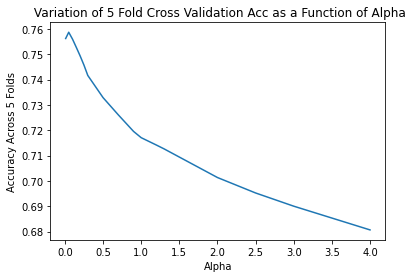
\includegraphics[width=\textwidth]{news-nb-hyperparamater-tuning.png}
    \caption{20 News Group Naive Bayes Hyperparameter Tuning}\label{news-nb-hyperparameter-tuning}
  \end{minipage}
\hspace{1.5cm}
 \begin{minipage}[h]{0.3\textwidth}
    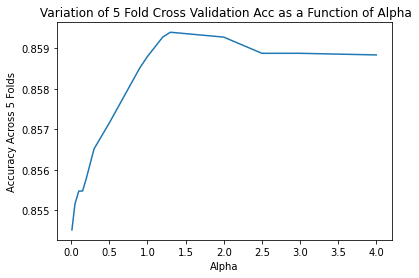
\includegraphics[width=\textwidth]{imdb-nb-hyperparamater-tuning.png}
    \caption{IMDB Naive Bayes Hyperparameter Tuning}\label{imdb-nb-hyperparameter-tuning}
  \end{minipage}
\end{figure}

\subsection{Accuracy Depending on Dataset Size}
We further compared the accuracy of the two models as a function of the size of the dataset by arbitrarily selecting 20\% intervals of the available training data to train our model on the 20 News Group set. Figures \ref{news-training-split-train} and \ref{news-training-split-test} plot our accuracies on the training set and test set respectively. The Naive Bayes performs consistently better on the testing set. Interestingly, logistic regression performs just as well and better than Naive Bayes for the testing set. 

Similarly, we ran this experiment for the IMDB Reviews set. Figures \ref{imdb-training-split-train} and \ref{imdb-training-split-test} plot our accuracies on the training set and test set respectively. As expected, we achieve higher accuracy as we train more of the dataset. Furthermore, Logistic Regression is consistently more accurate especially for a larger dataset as it is a discriminative algorithm. 

\begin{figure}[h!]
  \centering
  \begin{minipage}[h]{0.3\textwidth}
    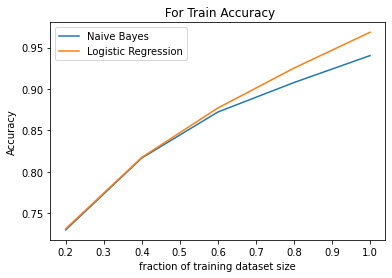
\includegraphics[width=\textwidth]{news-varying-train-set-size-train-accuracy.png}
    \caption{News Training Accuracy Based on Training Set Split }\label{news-training-split-train}
  \end{minipage}
\hspace{1.5cm}
   \begin{minipage}[h]{0.3\textwidth}
    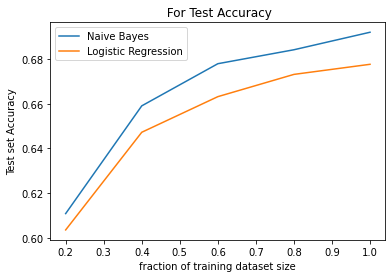
\includegraphics[width=\textwidth]{news-varying-train-set-size-test-accuracy.png}
    \caption{News Testing Accuracy Based on Training Set Split}\label{news-training-split-test}
  \end{minipage}
\end{figure}

\begin{figure}[h!]
  \centering
  \begin{minipage}[h]{0.3\textwidth}
    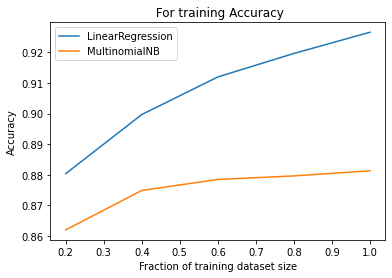
\includegraphics[width=\textwidth]{imdb-varying-train-set-size-train-accuracy.png}
    \caption{IMDB Training Accuracy Based on Training Set Split}\label{imdb-training-split-train}
  \end{minipage}
\hspace{1.5cm}
   \begin{minipage}[h]{0.3\textwidth}
    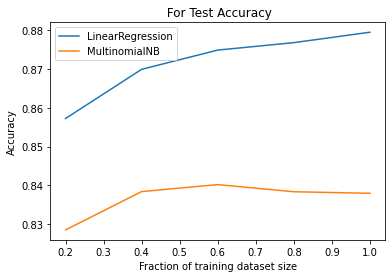
\includegraphics[width=\textwidth]{imdb-varying-train-set-size-test-accuracy.png}
    \caption{IMDB Testing Accuracy Based on Training Set Split}\label{imdb-training-split-test}
  \end{minipage}
\end{figure}

\subsection{Comparison with Other Models}
Table \ref{table-models} presents the models we used on both datasets. In addition to the Naive Bayes and Logistic Regression classifiers, we looked into SGDC (SVM since loss = hinge), Decision Trees, and Ada Boost to test how they would perform on our datasets. SVMs (Support Vector Machines) are some of the best natural language processing tools in the industry, especially the ones with linear kernels. Therefore, we suspected it would perform well on our sets. Furthermore, we previously used the decision tree classifier and found it effective, so we tested it as well. We conclude that for the 20 News Group dataset, our Naive Bayes model still performs the best, whereas SGDC is slightly better than logistic regression. Even more, it is the fastest classifier for training. The decision tree classifier has the highest training accuracy (most overfit). On the other hand, for the IMDB dataset, the Logistic Regression model is still the most accurate. It is also the fastest model for training on the dataset. As with the news dataset, the decision tree classifier once again has the highest training accuracy. 


\begin{table}[h!] 
\centering
\begin{tabular}{||c c c c c||} 
 \hline
 Classifier & Dataset & Best Train Accuracy (\%) & Best Test Accuracy (\%) & Time (s)\\ [0.5ex] 
 \hline\hline
 \rowcolor{lightgray}Naive Bayes && 94.03 & 69.20 & 17.56 \\ 
 Logistic Regression && 74.54 & 67.30 & 182.60 \\
 SGDC & 20 News Group & 89.33 & 67.90 & 6.02 \\
 Decision Tree && 97.23 & 44.07 & 418.96 \\
  Ada Boost && 41.32 & 36.36 & 261.75\\
 \hline \hline
 Naive Bayes && 88.19 & 83.65 & 5.53 \\
\rowcolor{lightgray}Logistic Regression && 92.66 & 87.95 & 2.64 \\
 SGDC & IMDB Reviews & 85.80 & 84.12 & 16.69 \\
 Decision Tree && 1.00 & 71.90 & 141.97 \\
 Ada Boost && 80.67 & 80.16 & 442.34 \\[1ex] 
 \hline
\end{tabular}
\caption{Comparing Various Models with Best Accuracies on both datasets}
\label{table-models}
\end{table}


\section{Discussion and Conclusion}
Based on our models and analyses, we conclude that the 20 News Group and IMDB Reviews datasets require different classifiers for the most accurate predictions since one is binary and one is multiclass. First, both datasets must be cleaned and vectorized using a TFIDF vectorizer in order to get the most accurate results and to reduce the training time significantly. The uncleaned set contains a lot of noise and unnecessary features. Using the cleaned set, for the 20 News Group data set, we achieved the best testing accuracy with our implementation of Multinomial Naive Bayes classifier. The logistic regression performed  on this set being less accurate and 10 times slower than Naive Bayes. Interestingly, our extra research showed that the SGDC classifier is almost 3 times faster than Naive Bayes while being slightly less accurate. The IMDB Reviews dataset had the best testing accuracy based off of the Logistic Regression Classifier. This model also trained faster, almost twice as fast as Naive Bayes while being about 4\% more accurate on the testing set.

\section{Statement of Contributions}
Arneet Singh Kalra wrote the maniuscript and assisted in developing K-fold cross validation. Behnaz Ghefati Feizabadi completed the analysis of the IMDB Reviews dataset. Hussein Lakkis developed the Naive Bayes model and did analysis of the 20 News Group dataset. 

\printbibliography
\end{document}